\documentclass[10pt]{beamer}

\usetheme[progressbar=frametitle]{metropolis}
\usepackage{appendixnumberbeamer}

\usepackage{booktabs}
\usepackage[scale=2]{ccicons}

\usepackage{pgfplots}
\usepgfplotslibrary{dateplot}

\usepackage{xspace}
\newcommand{\themename}{\textbf{\textsc{metropolis}}\xspace}

\title{Cryptographie}
\subtitle{UE OP6.33}
% \date{\today}
\date{\today}
\author{Nour Boulahcen}
\institute{Institut Villebon Georges Charpak}

\titlegraphic{\hfill
\includegraphics[height=2.5cm]{logo.png}}

\begin{document}

\maketitle

\begin{frame}{Table of contents}
  \setbeamertemplate{section in toc}[sections numbered]
  \tableofcontents%[hideallsubsections]
\end{frame}

\section{Introduction}

\begin{frame}[fragile]{Demarche}

  Le but de cette UE était de décoder 8 messages et chacun de ces messages nous donne une information sur comment a été chiffré le message suivant. Cela nous a amené a devoir implenter 4 chiffres: 
  \begin{itemize}
      \item \textsc{Scytale}
      \item \textsc{Caesar}
      \item \textsc{Vigenere}
      \item \textsc{Enigma}
  \end{itemize}
\end{frame}


\section[Chiffre par transposition - \large{\texttt{\textit{Scytale}}}]{Chiffre par transposition}

\begin{frame}{Implementation}
    \begin{figure}
        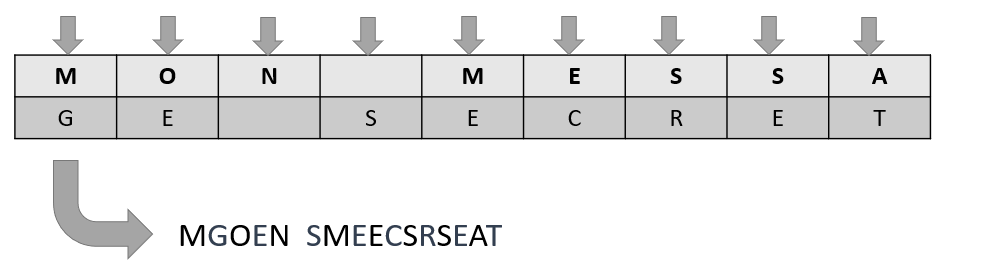
\includegraphics[scale=0.45]{scytale1.PNG}
         \caption{Chiffrement par Scytale}
  \end{figure}
 
\end{frame}
\begin{frame}{Implementation}
    \begin{figure}
        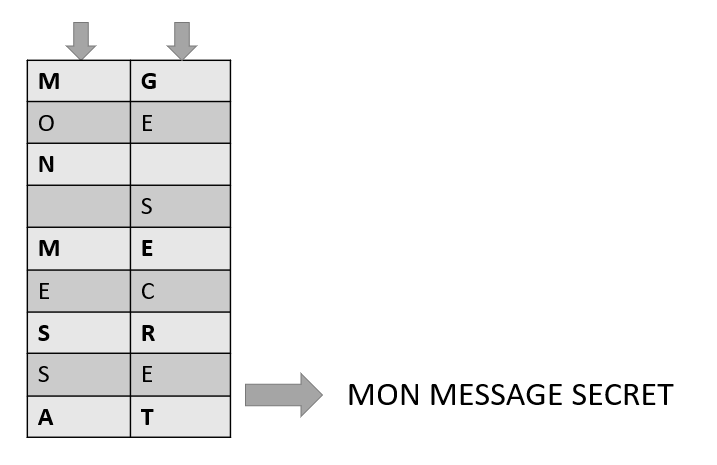
\includegraphics[scale=0.45]{scytale2.PNG}
        \caption{Dechiffrement par Scytale}
  \end{figure}
  
\end{frame}



{
    \metroset{titleformat frame=smallcaps}
\begin{frame}{Attaque}
\alert{\texttt{\textbf{Attaque Brutforce}}}
	\begin{itemize}
    \item \textsc{Autant de tentative que de caractère}
    \item \textsc{Filtre par \textbf{mot clé} (Joël)}
    \item \textsc{S'arrête quand le mot clé est trouvé}
    \item \texttt{\textbf{Complexité en  $O(n^2(n+1)/2 + n)$}}

  \end{itemize}
\end{frame}
}

\section[Chiffre par substitution - \large{\texttt{\textit{César/Vigenere}}}]{Chiffre par substitution}

\begin{frame}{Implementation}
    \begin{figure}
        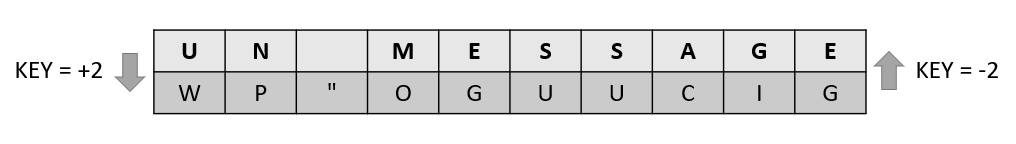
\includegraphics[scale=0.42]{caesar.PNG}
        \caption{Chiffre de Caesar}
  \end{figure}
 
\end{frame}
\begin{frame}{Implementation}
    \begin{figure}
        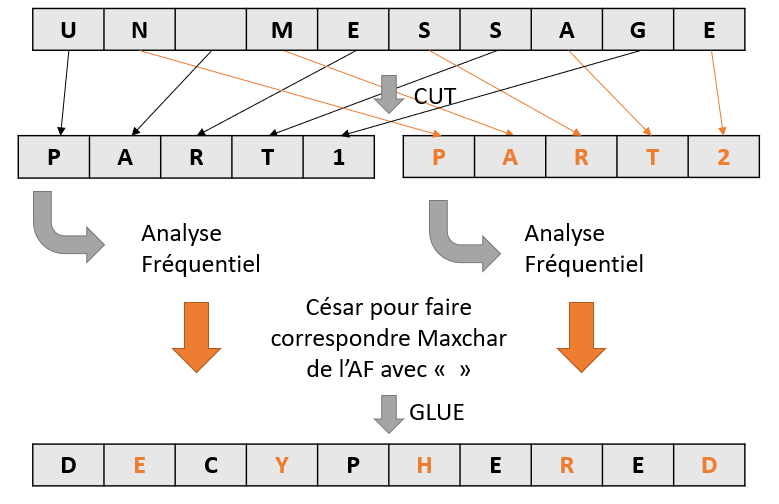
\includegraphics[scale=0.45]{vigenere.PNG}
        \caption{Chiffre de Vigenere}
  \end{figure}
  
\end{frame}

{
    \metroset{titleformat frame=smallcaps}
\begin{frame}{Attaque}
\alert{\texttt{\textbf{Attaque Brutforce}}}
	\begin{itemize}
    \item \textsc{Autant de tentative que de caractère (attaque sur la découpe)}
    \item \textsc{On essaie de deviner le décalage du césar par \textbf{AF}}
    \item \textsc{Pour que l'AF soit efficace, le texte doit être \textbf{assez long}}
    \item \textsc{Filtre par \textbf{mot clé} (Joël)}
    \item \textsc{S'arrête quand le mot clé est trouvé}
    \item \texttt{\textbf{Complexité en  $O(n^4 + n^3 + n^2 + n)$}}

  \end{itemize}
\end{frame}
}


\section[\Large{\texttt{\textit{Enigma}}}]{Enigma}


\begin{frame}{Implementation}
    \begin{figure}
        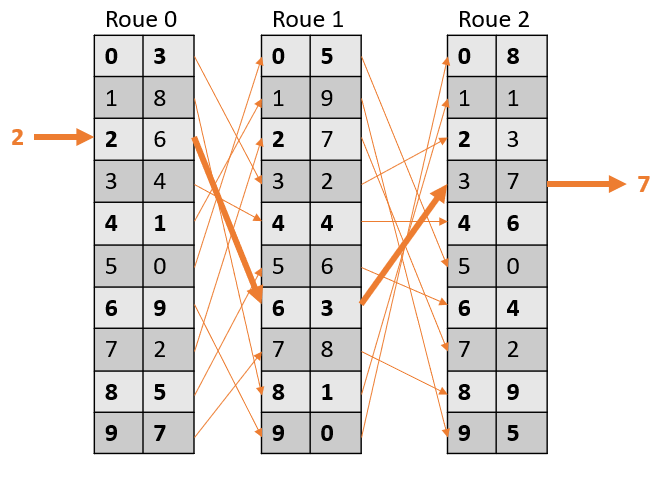
\includegraphics[scale=0.5]{Enigma.PNG}
        \caption{Encodage d'un caractère par Enigma}
  \end{figure}
  
\end{frame}
\begin{frame}{Implementation}
    \begin{itemize}
        \item Pour chaque caractère, la roue 0 tourne d'un cran
        \item Pour chaque tour complet de la roue 0, la roue 1 tourne d'un cran
        \item Pour chaque tour complet de la roue 1, la roue 2 tourne d'un cran
    \end{itemize}
  
\end{frame}
\begin{frame}{Implementation}
    Faire tourner les roues et encoder le caractère est équivalent a faire tourner le carctère l'encoder puis de le faire tourner dans l'autre sens : $ABA^-1 \equiv B$  
  
\end{frame}
\begin{frame}{Implementation}
    \begin{figure}
        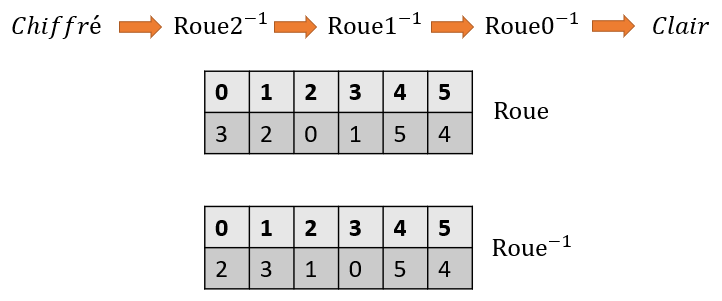
\includegraphics[scale=0.5]{enigma2.PNG}
        \caption{Décodage d'un texte par Enigma}
  \end{figure}
  
\end{frame}

\begin{frame}{Attaque}
  \alert{\texttt{\textbf{Attaque Brutforce}}}
	\begin{itemize}
    \item \textsc{On a 3 parmis 8 combinaisons de roues et 3 parmis 256 position initale }
    \item \textsc{Supposition:} le premier mot du message est "Félicitation"
    \item \textsc{On brutforce donc uniquement les 13 premiers char pour trouver la clé}
    \item \textsc{Une fois la clé trouvé, on peut décrypter le message entier}
    \item \textsc{Pour plus de rapidité pour le brutforce, on pourait l'implementer en C}

  \end{itemize}
\end{frame}






{\setbeamercolor{palette primary}{fg=black, bg=yellow}
\begin{frame}[standout]
  Questions?
\end{frame}
}

\appendix

\end{document}
